\documentclass[12pt]{article}

\addtolength{\textwidth}{1.3in}
\addtolength{\oddsidemargin}{-.65in} %left margin
\addtolength{\evensidemargin}{-.65in}
\setlength{\textheight}{9in}
\setlength{\topmargin}{-.5in}
\setlength{\headheight}{0.0in}
\setlength{\footskip}{.375in}
\renewcommand{\baselinestretch}{1.0}
\renewcommand{\thesection}{\Roman{section}} 
\renewcommand{\thesubsection}{\thesection.\Alph{subsection}}
\linespread{1.5}

\usepackage[pdftex,
bookmarks=true,
bookmarksnumbered=false,
pdfview=fitH,
bookmarksopen=true]{hyperref}
\usepackage[pdftex]{graphicx}
%\usepackage{pdfpages}

\usepackage[usenames,dvipsnames,svgnames,table]{xcolor}
\usepackage{cite}
\usepackage{times, verbatim,bm,pifont,pdfsync}
%\usepackage[hang,flushmargin]{footmisc}%unindents footnotes

% disables chapter, section and subsection numbering
%\setcounter{secnumdepth}{-1} 

\usepackage{amsbsy,amssymb, amsmath, amsthm, MnSymbol,bbding}
\usepackage[hang,flushmargin]{footmisc} 

\newtheorem{definition}{Definition}
\newtheorem{theorem}{Theorem}
\newtheorem{lemma}{Lemma}
\newtheorem{corollary}{Corollary}
\newtheorem{assumption}{Assumption}
\newtheorem{fact}{Fact}
\newtheorem{result}{Result}
\newtheorem{proposition}{Proposition}

\newcommand{\ve}{\theta}
\newcommand{\ta}{\theta}
\newcommand{\ov}{\overline}
\newcommand{\un}{\underline}
\newcommand{\al}{\alpha}
\newcommand{\Ta}{\Theta}
\newcommand{\expect}{\mathbb{E}}
\newcommand{\Bt}{B(\bm{\tau^a})}
\newcommand{\bta}{\bm{\tau^a}}
\newcommand{\bte}{\bm{\tau^E}}
\newcommand{\btn}{\bm{\tau^n}}
\newcommand{\ga}{\gamma}


\begin{document}
\title{\vskip-0.6in LOBBYING AND LEGISLATIVE UNCERTAINTY}
\author{Kristy Buzard\thanks{Syracuse University, Economics Department, 110 Eggers Hall, Syracuse, NY 13244. Ph: 315-443-4079. Fax: 315-443-3717. Email: kbuzard@syr.edu. http://faculty.maxwell.syr.edu/kbuzard.} \and Sebastian Saiegh\thanks{University of California, San Diego, Department of Political Science, Social Sciences Building 365, 9500 Gilman Drive, La Jolla, CA 92093. Ph: 858-534-7237. Fax: 858-534-7130. Email: ssaiegh@ucsd.edu. http://pages.ucsd.edu/~ssaiegh/.}} 
\date{\vskip-.1in \today}
\maketitle

\begin{center} {\bf Abstract} \end{center}

\begin{quote}
{This paper seeks to understand how uncertainty affects the incentives for lobbying and the associated prospects for the passage of legislation. We introduce a model of vote buying in which there is uncertainty about the ideological positions of legislators with information about this uncertainty symmetric among all players. When legislators' voting behavior cannot be perfectly anticipated in this manner, the model is able to describe various realistic aspects of lobbying and voting behavior. For example, it predicts that lobbyists on both sides of an issue may be active at the same time, that moderate legislators and those about which there is average uncertainty receive more bribes than those that are ideologically extreme, and that ideal points gross of bribes need not be equalized. Estimating ideal points using a logistic item response model, we find support for these predictions in U.S. House of Representatives roll call data.

\textit{JEL classification:} D72, D80, C72 \\
\textit{Keywords:} lobbying, political economy, legislatures, uncertainty}
\end{quote}

\bigskip
\section{Introduction}
\label{sec:intro}

In the United States alone, nearly $4$ billion dollars is spent every year on lobbying and campaign contributions. Looking at the U.S. Congress, for instance, we see that special interest groups exert these economically significant amounts of effort and resources to influence a legislative process that is fraught with uncertainty. In particular, legislators' voting behavior can seldom be perfectly anticipated, as lawmakers consider a variety of influences when deciding how to vote, including their personal values, announced positions, the views of their constituents, and the preferences of their party leadership.

Saiegh (2011) identifies two major factors that shape lawmaking: whether buying legislative votes is a feasible option and the unpredictability of legislators' voting behavior. When vote buying is possible and legislative uncertainty is present---as is often the case---the optimal lobbying strategies are far from obvious. This paper seeks to understand how uncertainty surrounding the preferences of legislators affects the incentives for lobbying and the associated prospects for the passage of legislation. 

We solve a model of vote buying in which there is uncertainty about the ideological positions of legislators. This model is able to describe some realistic aspects of lobbying and voting behavior: for instance, it predicts that lobbyists on both sides of an issue may be active at the same time, that moderate legislators and those about which there is average uncertainty receive more bribes than those that are ideologically extreme, and that ideal points gross of bribes need not be equalized. We find support for these predictions in U.S. House of Representatives roll call data, from which we estimate ideal points using a logistic item response model.

In constructing the model, we follow Groseclose and Snyder (1996) and Banks (2000) in taking a policy proposal as given and studying the behavior of interest groups who may lobby legislators in an attempt to sway the outcome of the vote. In order to keep the model tractable, we study a three-person legislature in which two lobbyists---one for the new proposal and one against it---sequentially offer payments to the legislators.

A payment to a legislator has the effect of shifting the legislator's ideal point, which we take to be known up to the mean and variance parameters of a given probability distribution. We assume that information about the legislators' ideal points is symmetric among all players; the legislators are not strategic and there is no motive for signalling. Bribing a legislator only has the effect of changing the probability with which the legislator votes in the manner the vote buyer prefers.

When the lobbyists are faced with this uncertainty about the preferences of the legislators, we find, quite intuitively, that the number of legislators a vote buyer chooses to lobby is increasing in the value he places on the policy. When a vote buyer's willingness-to-pay for his preferred policy is very low, he will bribe none of the legislators; if it is very high, he will bribe all of them. Intermediate outcomes are also possible.

Perhaps more interesting, and in contrast to results in a model without uncertainty, when only one or two legislators are bribed the legislator who remains unbribed is often the one who is most ideologically-aligned with the vote buyer. When the legislators are roughly unbiased on average, it is the moderate legislator who is bribed first. This corresponds well with the data that shows that more moderate legislators receive more campaign contributions.

If we assume identical levels of uncertainty about the ideal points of all the legislators, we find that the vote buyers use `leveling strategies' as in Groseclose and Snyder (1996) and Banks (2000). Allowing for asymmetric levels of uncertainty, on the other hand, provides a more realistic picture that accords well with our empirical findings that legislators with moderate levels of uncertainty are the target of the highest levels of lobbying, while those about whom there are very high levels of uncertainty most often remain unbribed.

We find one more result that is appealing from an empirical point of view. In models of vote buying that do not incorporate uncertainty, only one vote buyer will pay bribes on any given issue. In this model with uncertainty about legislators' ideal points, however, it is possible to have both vote buyers paying positive bribes on the same issue. The results of the model accord well with these important patterns in the data, and we believe this model makes an important contribution to the understanding of the political uncertainty that surrounds statutory lawmaking. It both brings more realism to the studying of legislative voting and vote buying \textit{and} gives us a window into an important, under-studied facet of the legislative environment.

Below we introduce an innovative methodology for quantifying cross-industry political uncertainty; the model under consideration here is being adapted as a means to properly identify political uncertainty in this context. We plan to establish the relevance of the resulting measures for policy-making and will make the data available for future use in a wide range of applications.

\subsection{Related Literature}
\label{sec:lit}

This work relates to the literature on vote-buying and legislative behavior in political science (Groseclose and Snyder (1996), Dekel et. al. (2005), Dal Bo (2007)) as well as to the canonical studies on endogenous regulation (cf. Stigler (1975), Peltzman (1976), Becker (1983), Laffont and Tirole (1994)).

Also related is Le Breton and Salanie (2003), which studies lobbying when the lobby is uncertain about the preferences of a unitary decision maker. Le Breton and Zaporozhets (2007) go a step further and replace the unitary decision maker with a legislature with multiple actors. Song (2008) is a model of endogenous lobbying with a ratification constraint in a context of unilateral policy making with no uncertainty, and Coates and Ludema (2001) study trade policy leadership in a model with endogenous lobbying in the presence of political uncertainty with imperfect monitoring.

As noted above, Saiegh (2009) argues that the uncertainty surrounding statutory lawmaking is in part related to governmental and political structure. Although they do not discuss uncertainty specifically, the cross-country empirical work of Gawande, Krishna and Olarreaga (2009) is the first to our knowledge that suggests that this kind of uncertainty plays a role in trade policy. They show that variables such as the number of checks and balances on the power of the legislature and the gap between the policy positions of the main political parties have predictive power for the PFS ``welfare-mindedness'' parameter. The model of Buzard (2016) indicates that the kind of political uncertainty modeled here can have an important impact on the formation and maintenance of trade agreements.

I will introduce the structural model in Section~\ref{sec:model} and discuss the theoretical results in Section~ \ref{sec:res}. Section~\ref{sec:est} discusses the estimation approach while Section~\ref{sec:house} applies this approach to the case of the U.S. House of Representatives. Section~\ref{sec:concl} concludes.


\section{The Model}
\label{sec:model}

The model is based on Banks' (2000) model of vote buying in a legislature, which is in turn a discrete version of Groseclose and Snyder's (1996) model with a continuum of legislators. The major difference here is the addition of uncertainty about the legislator's ideal points.

Each of three legislators faces a choice between the status quo, $x$ and a new policy proposal $s$. The utility function of legislator $i$ is given by $v(i) = u_i(x) - u_i(s)$, which is measured in money units. Note that legislators only have preferences about how they vote, not over which alternative wins.

There are two vote buyers labeled $A$ and $B$ who each prefers to maximize the expected value of his preferred policy net of the bribes he has to pay. $A$ prefers policy $x$ and has willingness to pay (WTP) $W_A$ for $x$ measured in money and values $s$ at zero. $B$ prefers $s$and has WTP $W_B$ for $s$. Each vote buyer would prefer to concede the issue rather than pay more than his WTP.

Vote Buyer $A$ moves first, providing a bribe offer function $a_i$. $a_i$ is perfectly observable to Vote Buyer $B$ when he moves second and offers bribe offer function $b_i$. Each legislator takes these bribe offers as given and then votes for the alternative that maximizes her payoff. I assume unbribed legislators who are indifferent vote for $s$.

\subsection{Legislature}
Let us look first at the legislature. Each legislator $i$ decides whether to vote for $x$ or $s$ given her preference $i$, $a_i$ and $b_i$. Although legislators are ordered on the interval according to their ideal points $i$, there is acknowledged uncertainty surrounding their preferences. We take this uncertainty to vary by legislator and also potentially by issue area when we extend the model to account for multi-dimensional voting and vote-buying.

In order to keep the model tractable when introducing this uncertainty, we take the ideal point function to be linear in $i$. That is, legislator $i$'s ideal point is taken to be $\alpha -\beta i$. We model uncertainty by taking legislator $i$ to vote for $x$ if 
			  \[
				  v(i) = \alpha -\beta i + \ve_i + a_i - b_i > 0
				\]
		
Notice that a bribe from $B$ is subtracted because it makes the alternative \textit{less} attractive.	We will begin by taking $\ve$ to not vary in $i$ and will shortly generalize.

Given these assumptions, the probability that legislator $i$ votes against the new proposal is
	\[
					\Pr\left[v(i)\leq 0 \right] = \Pr\left[\alpha -\beta i + \ve + a_i - b_i \leq 0 \right] = \Pr\left[\ve \leq \beta z - \alpha - a_i + b_i \right] 
	\]
Assuming $\ve \sim \text{Logistic} \ (0,1)$, the probability that legislator $z$ votes ``no'' is $\frac{1}{1+e^{-\left(\beta i - \alpha - a_i + b_i \right)}}$.	Whether a legislator $i$ votes ``no'' is a random variable, denote it $Q(i)$, distributed Bernoulli with this probability:
	\[
		Q(i) \sim \text{Bernoulli}(p(z)) \hskip.2in \text{where} \hskip.2in p(z) = \frac{1}{1+e^{-\left(\beta z - \alpha -a_i+ b_i \right)}}
	\]

For ease of exposition, for now take $i \in \left\{ -\frac{1}{2}, 0, \frac{1}{2} \right\}$. Then $Y_B = \frac{\beta}{2} - \alpha - a_{-\frac{1}{2}} + b_{-\frac{1}{2}}$, $X_B = -\alpha - a_0+ b_0$ and $Z_B = -\frac{\beta}{2} - \alpha - a_{\frac{1}{2}} + b_{\frac{1}{2}}\label{page:sh}$ represent the net ideal points in terms of $B$'s probability of winning the issue. We can then write the probability that each of the legislators, respectively, votes against the new proposal as $\frac{1}{1+e^{-Y_B}}$, $\frac{1}{1+e^{-X_B}}$ and $\frac{1}{1+e^{-Z_B}}$.

Vote Buyer $A$ must take into account that Vote Buyer $B$ will react to her choice of bribes. So the net ideal points from her point of view---that is, in terms of her winning the issue---are $X_A = \alpha - b_0(\bm{a},W_B,\al,\beta) + a_0$, $Y_A = -\frac{\beta}{2} + \alpha - b_{-.5}\left(\bm{a},W_B,\al,\beta\right)+ a_{-.5}$, and $Z_A = \frac{\beta}{2} + \alpha - b_{.5}\left(\bm{a},W_B,\al,\beta\right)+ a_{.5}$ with $\bm a = \left(a_{-.5},a_0,a_{.5} \right)$. We can then write the probability that each of the legislators votes for the new proposal as $\frac{1}{1+e^{-Y_A}}$, $\frac{1}{1+e^{-X_A}}$ and $\frac{1}{1+e^{-Z_A}}$.
				

\subsection{Vote Buyer B}
Groseclose and Snyder (1996) assume that the objective of each vote buyer is to ``minimize total bribes paid while passing his preferred policy.'' This has to be adapted out our environment with uncertainty about legislators' ideal points, as with any probability distribution with infinite support both players will necessarily have a positive probability of winning in equilibrium regardless of their strategies. The appropriate analog is that vote buyers maximize the expected value of winning the vote net of bribes that he/she must pay. Note that in order to maximize the probability of winning a majority in a three-seat legislature, one must maximize the probability of at least two legislators voting with you. The case of Vote Buyer $B$, this is the probability that at least two legislators vote in favor of the status quo: $\Pr(S \geq 2)$ where $S = X\left(-\frac{1}{2}\right) + X\left(0\right) + X\left(\frac{1}{2}\right)$.

This means that the maximization problem for Vote Buyer B (in absence of Vote Buyer A) is
			  \begin{multline}
			    \max_{b_{-\frac{1}{2}}, b_0, b_{\frac{1}{2}}} 
					W_B \biggl[ \Pr\left(X\left(-\frac{1}{2}\right)=1\right)\Pr\left(X\left(0\right)=1\right)\left(X\left(\frac{1}{2}\right)=0\right)  + \\
					\Pr\left(X\left(-\frac{1}{2}\right)=1\right)\Pr\left(X\left(0\right)=0\right)\Pr\left(X\left(\frac{1}{2}\right)=1\right) + \\
					\Pr\left(X\left(-\frac{1}{2}\right)=0\right)\Pr\left(X\left(0\right)=1\right)\Pr\left(X\left(\frac{1}{2}\right)=1\right) + \\
					\Pr\left(X\left(-\frac{1}{2}\right)=1\right)\Pr\left(X\left(0\right)=1\right)\Pr\left(X\left(\frac{1}{2}\right)=1\right) \biggr] - \sum_{j\in \left\{-\frac{1}{2}, 0,\frac{1}{2}\right\}} b_j
				\end{multline}
			Substituting from the definition of $X$,
			  \begin{multline}
			    \max_{b_{-\frac{1}{2}}, b_0, b_{\frac{1}{2}}} 
					W_B \biggl[ \frac{1}{1+e^{-Z}} \frac{1}{1+e^{-X}} \left(1-\frac{1}{1+e^{-Y}}\right)  + \\
					\frac{1}{1+e^{-Z}} \left(1-\frac{1}{1+e^{-X}}\right) \frac{1}{1+e^{-Y}} + \\
					\left(1-\frac{1}{1+e^{-Z}} \right) \frac{1}{1+e^{-X}} \frac{1}{1+e^{-Y}} + \\
					\frac{1}{1+e^{-Z}} \frac{1}{1+e^{-X}} \frac{1}{1+e^{-Y}} \biggr] - \sum_{j\in \left\{-\frac{1}{2}, 0,\frac{1}{2}\right\}} b_j
				\end{multline}
			This can be simplified as 
			  \begin{multline}
			    \max_{b_{-\frac{1}{2}}, b_0, b_{\frac{1}{2}}} 
					W_B \biggl[ \frac{1}{1+e^{-X}} \frac{1}{1+e^{-Y}} +
					\frac{1}{1+e^{-X}} \frac{1}{1+e^{-Z}} + \\
					\frac{1}{1+e^{-Y}} \frac{1}{1+e^{-Z}} - 2	\frac{1}{1+e^{-Z}} \frac{1}{1+e^{-X}} \frac{1}{1+e^{-Y}} \biggr] - \sum_{j\in \left\{-\frac{1}{2}, 0,\frac{1}{2}\right\}} b_j
					\label{eq:objb}
				\end{multline}
		
\subsection{Vote Buyer A}
Vote buyer A's objective function is identical in form to that of Vote buyer B (Expression~\ref{eq:objb}) 
			  \begin{multline}
			    \max_{a_{-\frac{1}{2}}, a_0, a_{\frac{1}{2}}} 
					W_A \biggl[ \frac{1}{1+e^{-X_A}} \frac{1}{1+e^{-Y_A}} +
					\frac{1}{1+e^{-X_A}} \frac{1}{1+e^{-Z_A}} + \\
					\frac{1}{1+e^{-Y_A}} \frac{1}{1+e^{-Z_A}} - 2	\frac{1}{1+e^{-Z_A}} \frac{1}{1+e^{-X_A}} \frac{1}{1+e^{-Y_A}} \biggr] - \sum_{j\in \left\{-\frac{1}{2}, 0,\frac{1}{2}\right\}} a_j .
					\label{eq:obja}
				\end{multline}

However, strategically Vote Buyer A is more complex because of the dependence of Vote Buyer $B$'s bids on her own.
				
\subsection{Non-negativity Constraints for Bribes}
\label{sec:nonneg}
It is not possible for a Vote Buyer to extract money from a legislator who is more favorably-inclined toward him than is optimal. This means that there are non-negativity constraints on all bribes. 

The Lagrangian for the problem is the same as Expression~\ref{eq:objb}, with the addition of three terms for the non-negativity constraints: $\lambda_X b_0 + \lambda_Y b_{-\frac{1}{2}} + \lambda_Z b_{\frac{1}{2}}$. Thus the full set of first order conditions are
\begin{equation}
    \frac{e^{-X}}{\left(1+e^{-X}\right)^2}\left[\frac{e^{-Z} + e^{-Y}}{\left(1+e^{-Z}\right)\left(1+e^{-Y}\right)} \right] = \frac{1 - \lambda_X}{W_B}
		\label{eq:focB}
\end{equation}
\begin{equation}
    \frac{e^{-Y}}{\left(1+e^{-Y}\right)^2}\left[\frac{e^{-X} + e^{-Z}}{\left(1+e^{-X}\right)\left(1+e^{-Z}\right)} \right] = \frac{1 - \lambda_Y}{W_B}
\end{equation}
\begin{equation}
    \frac{e^{-Z}}{\left(1+e^{-Z}\right)^2}\left[\frac{e^{-X} + e^{-Y}}{\left(1+e^{-X}\right)\left(1+e^{-Y}\right)} \right] = \frac{1 - \lambda_Z}{W_B}
\end{equation}
\[
  b\left(0\right) \geq0 \hskip.2in b\left(\frac{1}{2}\right) \geq0 \hskip.2in b\left(-\frac{1}{2}\right) \geq0 
\]
\[
  \lambda_X \geq0 \hskip.2in \lambda_Y \geq0 \hskip.2in \lambda_Z \geq0 
\]
\[
  \lambda_X \cdot b\left(0\right) = 0 \hskip.2in \lambda_Y \cdot b\left(-\frac{1}{2}\right) = 0 \hskip.2in \lambda_Z \cdot b\left(\frac{1}{2}\right) = 0 
\]



\subsection{Varying Uncertainty across Legislators}
\label{sec:uncert}
We allow the amount of uncertainty regarding each legislator's ideal point to vary across legislators by letting the scale parameter of the logistic distribution be different for each legislator. A larger scale parameter is associated with greater variance and thus more uncertainty as to the legislator's ideal point. The objective function for Vote Buyer $B$ becomes
 \begin{multline}
    \max_{b_{-\frac{1}{2}}, b_0, b_{\frac{1}{2}}} 
					W_B \biggl[ \frac{1}{1+e^{-\frac{X}{s_0}}} \frac{1}{1+e^{-\frac{Y}{s_{-.5}}}} +
					\frac{1}{1+e^{-\frac{X}{s_0}}} \frac{1}{1+e^{-\frac{Z}{s_{.5}}}} + \\
					\frac{1}{1+e^{-\frac{Y}{s_{-.5}}}} \frac{1}{1+e^{-\frac{Z}{s_{.5}}}} - 2	\frac{1}{1+e^{-\frac{Y}{s_{-.5}}}} \frac{1}{1+e^{-\frac{X}{s_0}}} \frac{1}{1+e^{-\frac{Z}{s_{.5}}}} \biggr] - \sum_{j\in \left\{-\frac{1}{2}, 0,\frac{1}{2}\right\}} b_j
	\end{multline}

We will see that allowing for this asymmetric uncertainty changes the predictions of the model in important ways. To lay the groundwork for the results to coming in Section~\ref{sec:resunc}, let's look at how the cumulative probabilities change for the most extreme legislators when the mean of their ideal point distribution is fixed but the scale parameter increases.

First, how does the probability that the legislator at $0.5$ (the one who is most unfriendly to $B$) votes with $B$ change when $s_{.5}$ goes from 1 to 2 in the absence of bribes? When $s_{.5}$ is 1, the probability is $\frac{1}{1+e^{-\frac{Z}{s_{.5}}}} = \frac{1}{1+e^{-\frac{-.5}{1}}} = \frac{1}{1+e^{.5}} = 0.3775$. When $s_{.5}$ is 2, the probability is $\frac{1}{1+e^{-\frac{Z}{s_{.5}}}} = \frac{1}{1+e^{-\frac{-.5}{2}}} = \frac{1}{1+e^{.25}} = 0.4378$. That is, the probability that the least friendly legislator votes with $B$ \textit{rises} when the uncertainty surrounding her ideal point increases.

Now, how does the probability that the legislator at $-0.5$ (the one who is most friendly to $B$) votes with $B$ change when $s_{-.5}$ goes from 1 to 2? When $s_{-.5}$ is 1, the probability is $\frac{1}{1+e^{-\frac{Y}{s_{-.5}}}} = \frac{1}{1+e^{-\frac{.5}{1}}} = \frac{1}{1+e^{-.5}} = 0.6225$. When $s_{-.5}$ is 2, the probability is $\frac{1}{1+e^{-\frac{Y}{s_{-.5}}}} = \frac{1}{1+e^{-\frac{.5}{2}}} = \frac{1}{1+e^{-.25}} = 0.5622$. Here, the probability that the most friendly legislator votes with $B$ \textit{falls} when the uncertainty surrounding her ideal point increases.



\section{Theoretical Results}
\label{sec:res}

Although uncertainty is present in the environment under consideration here, information about that uncertainty is symmetric. Therefore the the solution concept employed here is subgame perfect Nash equilibrium.

Whenever there is a possibility of multiple equilibria, I will focus on the one that maximizes the welfare of Vote Buyer A, the first mover.


\subsection{Vote Buyer B}
\label{sec:resB}

I begin by examining the subgame that begins when Vote Buyer $B$ makes his offer. This not only serves to elucidate the basic logic of the model; it will also serve as a baseline from which to examine the incentives of Vote Buyer $A$. These results also represent the outcomes when $A$'s willingness to pay is low, in which case it refrains from lobbying altogether and $B$'s incentives are the same as if Vote Buyer $A$ did not exist. For now, assume that the uncertainty about ideal points is the same across legislators.

In a legislature with three voters, Vote Buyer $B$ can choose to bribe all three legislators, two, one or none of the legislators. It is most instructive to begin with the case where he bribes two of the legislators.

\begin{proposition}
  When Vote Buyer $B$ pays bribes to exactly two legislators, the bribes are such that the two bribed legislators' ideal points gross of bribes are equalized. Which two legislators are bribed depends on the bias parameter $\al$.
	\label{prop:2NNB}
\end{proposition}

All proofs are in the Appendix.

The first part of this result is similar in spirit to Groseclose and Snyder (1996) and Banks (2000) in that a `leveling' strategy is employed. But the non-negativity constraint here binds for the third, and which legislator is this third, un-bribed legislator depends on where the three ideal points are relative to the zero point at which a legislator has a 50$\%$ probability of voting for either the status quo or the new proposal. If $B$'s willingness-to-pay parameter increases, the non-negativity constraint becomes less binding. That is, when Vote Buyer $B$'s willingness to pay becomes high enough, the additional probability of winning gained by bribing the third legislator becomes worth the additional cost. When this happens, he finds himself in the following case.

\begin{proposition}
  When Vote Buyer $B$ pays bribes to all three legislators, the bribes are such that the legislators' ideal points gross of bribes are equalized.
	\label{prop:3NNB}
\end{proposition}

This has the feel of Groseclose and Snyder (1996) and Banks (2000) but the logic is different. There, gross ideal points are equalized so that there is no wasted expenditure, as the second mover would ignore whichever voter was most expensive to him. In contrast, these results are in the context of only one lobby buying votes: it equalizes the legislators' gross positions because the probability density functions are unimodal and the marginal value of a bribe should be the same across all bribed legislators. If the ideal points are very close, it would be sub-optimal to continue moving one legislator and leave the other behind: the marginal increase would be greater for whichever legislator's ideal point is to the left once both have achieved a gross position greater than zero.


\begin{proposition}
  When Vote Buyer $B$ pays bribes to exactly one legislator, it may be any one of the three legislators depending on the bias parameter $\al$.
	\label{prop:1NNB}
\end{proposition}
In contrast to models with no uncertainty about legislators' ideological positions, here we have an anti-result that the vote buyers do not necessarily bribe those who are ideologically most aligned with themselves. The non-negativity constraint often rules out bribing the most friendly legislator(s) because she/they don't contribute very much to the overall probability of winning the issue. In fact, if it were possible, the vote buyer would often like to be paid by the most friendly legislator in exchange for her moving away from his position; that is, the most friendly legislator is often well past the point of optimality were the vote buyer to pay a bribe.

Figure~\ref{fig:br} shows an example of a vote in which the most money went to the ideologically moderate--not the most extreme in a `leveling' strategy.

Finally, for completeness we state a somewhat obvious result concerning the final possible case:

\begin{proposition}
  When Vote Buyer $B$ has a low willingness to pay, he does not bribe any legislator.
	\label{prop:0NNB}
\end{proposition}

When $W_B$ is low enough, the non-negativity constraint binds for all three legislators and Vote Buyer $B$ finds it in his interest to take his chances with the ideal point distributions as they stand.


\subsection{Varying Uncertainty across Legislators}
\label{sec:resunc}

The results of Section~\ref{sec:resB} in which bribed legislators have their ideal points `leveled' so that their positions gross of bribes are equalized hinge on assumption that the uncertainty surrounding the ideal points of each legislator is the same. The results become more interesting and more realistic if we allow for asymmetry in the uncertainty surrounding legislators' ideal points.

\begin{proposition}
  When there is no bias in the positions of the legislators ($\al =0$), the bribes of legislators whose ideal points are at the median in terms of uncertainty receive the highest relative bribes. [conjecture]
	\label{prop:asym}
\end{proposition}
In numerical examples, this pattern holds strongly. By `relative,' we mean that the bribes are scaled up relative to the bribe profile that creates equal gross position when uncertainty is symmetric. We also see that the bribes for legislators whose ideal points are more uncertain are scaled down while the bribes of legislators whose ideal points are less uncertain are scaled up, modulo relative position. That is, there is some effect of being more friendly versus less friendly, as the cumulative density that the legislator will vote in the vote buyer's favor changes in opposite directions when uncertainty rises depending on whether the legislator is friendly or unfriendly (cfr Section~\ref{sec:uncert}). This accords well with the finding in Figure \ref{fig:g1} that those legislators with very low and very high uncertainty get the lowest payments, while those with more average levels of uncertainty receive the most.

We demonstrate via the following numerical example. Let there be no bias on average in the un-bribed positions of the legislators (i.e. set the bias parameter at $\al=0$) and ignore Vote Buyer A. When we increase the scale parameter $s_{.5}$ for the legislator at $0.5$---that is, the least friendly to Vote Buyer $B$---from 1 to 1.5, $B$ stops bribing the most friendly legislator altogether. Vote Buyer $B$ does better in welfare terms because the probability that this legislator votes in his favor shifts upward. In fact, $s_{.5}$ must be much closer to $1$ in order for $B$ to bribe this legislator, and when he does, the gross ideal point is smaller in absolute value than that for the other two legislators.

On the other hand, if $s_{.5}$ is reduced from 1 to $0.75$, for an intermediate range of the willingness to pay parameter $W_B$, Vote Buyer $B$ switches to \textit{only} bribing legislator $0.5$. As $W_B$ increases, eventually all three legislators are bribed again, but now this legislator receives a larger gross bribe.

Recall that the effects are not necessarily entirely symmetric for the two extreme legislators because increasing uncertainty has an opposite effect on how much probability mass is above or below zero. However, there are strong similarities here. As $s_{-.5}$ is increased from 1 to 1.5 or larger, $B$ stops bribing this most friendly legislator and the asymmetry has to be reduced to below 1.2 in order for him to resume bribing legislator $-0.5$. When he does so, he will move this legislator less than the other two legislators about whom there is less uncertainty. If we instead reduce $-0.5$'s uncertainty, Vote Buyer $B$ moves this legislator further than the other two.
		
		
\subsection{Two Vote Buyers}
\label{sec:two}
Now we consider the entire game by adding Vote Buyer $A$'s choice of bribes. Vote Buyer A's first order conditions are more complicated than those of Vote Buyer $B$ because her choices $\bm a$ will impact those of Vote Buyer $B$.

Below is the first order condition with respect to $a_0$, which can be compared to Equation~\ref{eq:focB} for Vote Buyer $B$:
			 \begin{multline}
					 \frac{e^{-X} + e^{-Z}}{\left(1+e^{-X}\right)\left(1+e^{-Z}\right)} \frac{e^{-Y}}{\left[1+e^{-Y}\right]^2} \frac{\partial b_{-.5}}{\partial a_0} + \\ 
					\frac{e^{-X} + e^{-Y}}{\left(1+e^{-X}\right)\left(1+e^{-Y}\right)} \frac{e^{-Z}}{\left[1+e^{-Z}\right]^2}\frac{\partial b_{.5}}{\partial a_0} + \\
					\frac{2+e^{-Y} + e^{-Z}}{\left(1+e^{-Y}\right)\left(1+e^{-Z}\right)} \frac{e^{-X}}{\left[1+e^{-X}\right]^2}\left[1 - \frac{\partial b_0}{\partial a_0} \right] = \frac{1 - \lambda_{XB}}{W_A}
					\label{eq:focA}
				\end{multline}

Unlike in models with no uncertainty, we do not have knife edge results in which Vote Buyer $A$ uses Vote Buyer $B$'s indifference condition to ensure that he buys no votes---there is no such indifference condition in the presence of uncertainty. However, it's possible that one or both vote buyers will not bribe any legislator because the non-negativity constraints bind for all three bribes. This requires that the willingness-to-pay parameters are sufficiently small for both vote buyers.
		
\begin{proposition}
  It is possible that neither vote buyer bribes any legislator on a given vote. This occurs when both vote buyers' willingness-to-pay parameters are small.
\end{proposition}

In many cases, Vote Buyer $A$ \textit{will} still find it optimal to bribe the legislators in such a manner than Vote Buyer $B$ does not counter any bribes. That is, its often optimal to choose $\bm a$ so that the partial derivatives of $B$'s bribes with respect to $a_0$ in Equation~\ref{eq:focA} are zero. This is not always the case with uncertainty, and especially in the case where uncertainty is asymmetric.

\begin{proposition}
  It is possible for both vote buyers to bribe legislators on the same vote.
	\label{prop:bothbribe}
\end{proposition}

This result in particular adds significant realism to the model predictions and will help to match the empirical patterns.
		
		
\section{Estimating Legislative Uncertainty}
\label{sec:est}

Recorded votes in legislatures (roll call data) are the most commonly used data source to measure politicians' spatial preferences. A well-established strategy is to use statistical techniques to represent patterns of legislative voting. The intuition behind these statistical models is that each roll call presents each legislator with a choice between a ``yea'' and a ``nay'' position. Legislators are presumed to vote for the position most similar to their own ideal policy position. As Clinton et al. (2004) note, it is possible to use Bayesian Markov chain simulation statistical methods to generate these preference estimates. This approach treats the unknown ideal points, bill parameters and legislators' utilities as random variables and condition upon the observed roll call data. The strategy is to impute values to these variables and estimate by regression the ideal points and bill parameters. The MCMC algorithm repeatedly performs these imputations and regressions and generates a large number of samples from the posterior density of the model parameters. Using this estimation procedure, we obtain summary statistics used for inference: legislators' mean and median ideal points as well as their 95$\%$ posterior confidence intervals. The latter are of particular interest to us, as we can use them to gauge the unpredictability of  legislators' voting behavior.

We are interested in unpredictability vis-a-vis particular policy issues. Poole (2005) suggests using subsets of roll calls to establish legislators' ideal points separately on each issue. Preliminary work with our data indicates that a more statistically-robust method is to use all roll call votes in a legislative session or group of sessions to estimate an ideal point that is multidimensional---that is, with one dimension for each interest group---allowing the partial pooling of information across roll calls. Multilevel modeling techniques, of which the standard ideal point estimation is a basic case, are perfectly suited to this task.

We therefore estimate the model
\begin{equation}
  \Pr(y_{kj} = 1) = \text{logit}^{-1}\left( \sum_{g=1}^G \ga_k^{(g)}\left( \alpha_j^{(g)} - \beta_k^{(g)}\right) \right)
	\label{eq:v2}
\end{equation}
with roll call votes numbered $k=1,\ldots,K$, legislators numbered $j=1,\dots,J$, and interest groups numbered $g=1,\dots,G$. $y_{jk}=1$ if legislator $j$ votes ``Yea'' on bill $k$; $y_{kj}=0$ if she votes ``Nay'' on bill $k$. Note that interest groups take positions on multiple roll call votes and different interest groups can take positions, often on opposing sides, on each vote.
		
This is a logistic item response (Rasch) model as adapted by Bafumi, et. al. (2005) to the legislative context. $\alpha_j^{(g)}$ is the ideal point of legislator $j$ on issue $g$ and $\beta_k^{(g)}$ is the ideal point of a legislator who is indifferent on vote $k$ for issue $g$. $\gamma_k^{(g)}$, the discrimination parameter, is a measure of the informativeness of issue $g$ for the vote on bill $k$: a large $\ga$ indicates that legislators are very likely to vote according to their preferences, whereas a small $\ga$ means that even significant margins of preference do not contribute much to the probability that legislators will vote in favor of the bill.

We are currently experimenting with some of the more sophisticated measures of uncertainty that are possible with a rich model such as this one; for instance the group mean for $\ga$ and constructs that combine model parameters.


\section{An Application to the U.S. House of Representatives}
\label{sec:house}
We look to voting patterns in the U.S. House of Representatives to see if the predictions of our model bear any resemblance to reality. We find suggestive preliminary evidence that adding uncertainty to a model of vote buying helps to understand observed patterns in the data and our next step is to pursue a better-identified model.


\subsection{Data}
Voting data will be obtained from Vote View, a website maintained by Professor Keith Poole (\url{http://voteview.com}). Details on each legislative proposal are available electronically through Thomas (\url{http://thomas.loc.gov}) and the sites of the House and Senate registrars.

We will use Maplight's contributions data, which provides evidence on public declarations by special interest groups to determine the relevant PAC contributions for the bills under consideration. In a related effort to better connect special interest activity to the intent of that activity, we will use data made available pursuant to the U.S. Lobbying Disclosure Act of 1995 and the Honest Leadership and Open Government Act of 2007 via the U.S. Senate Office of Public Records and the Office of the Clerk of the U.S. House of Representatives. This data is particularly useful because lobbyists must declare the issue area on which they lobbied.

We will also explore whether there is a way to leverage the data and methodology of Lake (2015) that combine the contributions and lobbying data to improve precision, although there is a concern about the coarseness of the data that must be overcome.

\subsection{Evidence}

\begin{figure}
\centering
\begin{minipage}{.5\textwidth}
  \centering
  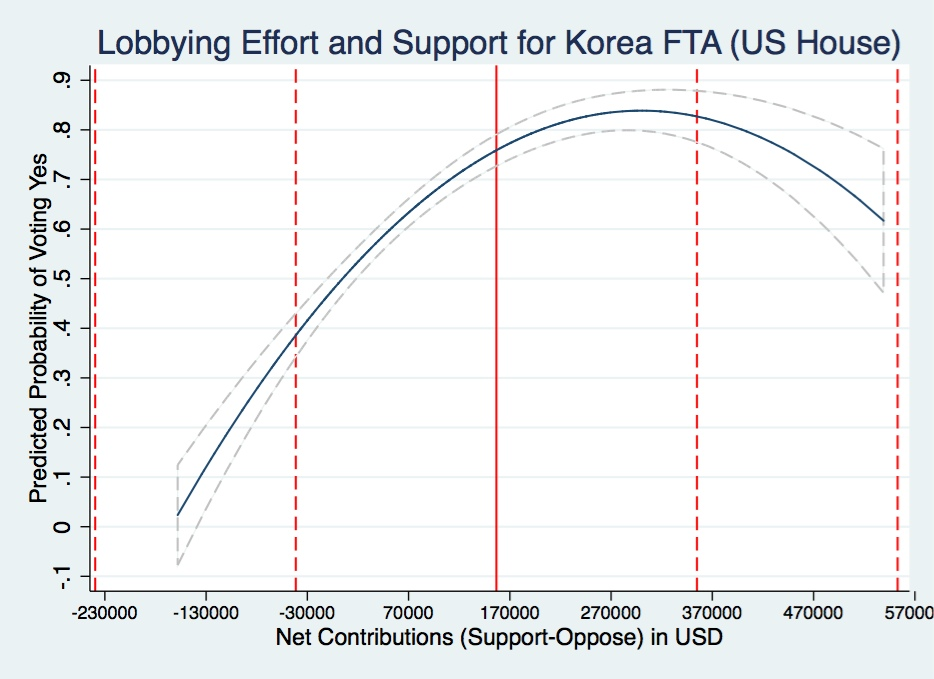
\includegraphics[width=2.9in]{graph2.jpg}
  \caption{\small Lobbying Effort and Support for KORUS
	\label{fig:br}}
\end{minipage}%
\begin{minipage}{.5\textwidth}
  \centering
  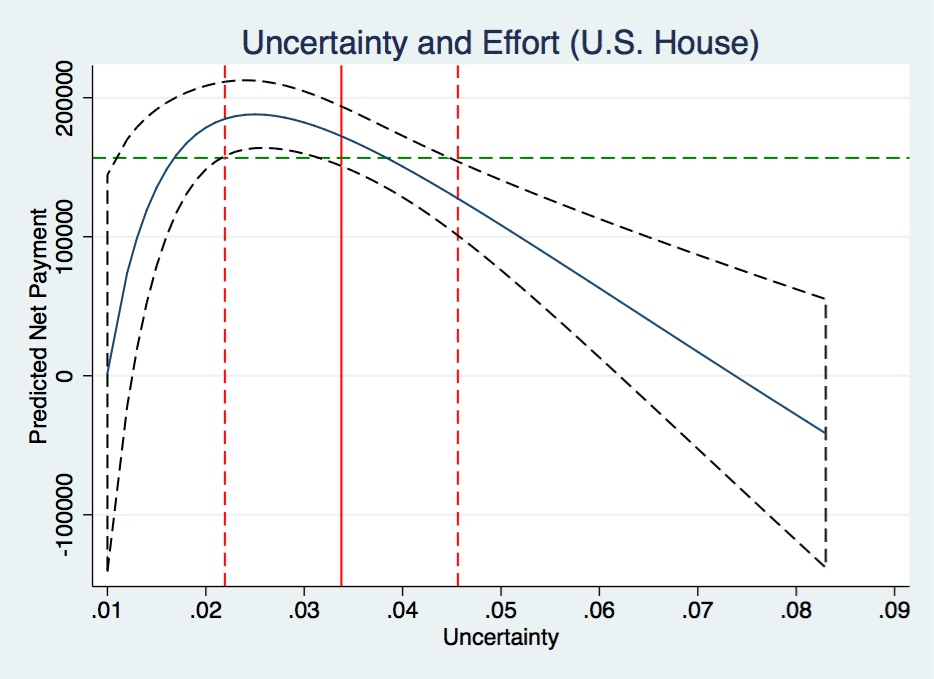
\includegraphics[width=2.9in]{graph1.jpg}
  \caption{\small Net Campaign Contributions, KORUS
	\label{fig:g1}}
\end{minipage}
\end{figure}

Figure~\ref{fig:br} displays the relationship between lobbying effort and legislators' support for one bill of interest, the Korea-U.S. Free Trade agreement, or KORUS. The vertical axis represents the predicted probability that a legislator would vote ``yes'' on the agreement, and the horizontal axis shows the monetary contributions to each legislator by lobbies who supported the passage of KORUS minus the contributions from lobbies opposing the agreement. The solid vertical red line indicates the average net contribution in the sample, and the dashed lines a one-standard deviation increase/decrease from that sample mean. To generate these results,  we regressed a legislator's vote on his/her estimated ideal point as well as partisanship using a probit specification. Then we fitted a second-order polynomial to the predicted probabilities generated by the probit regression. The contribution data for both this and the following figure was obtained from Maplight. The data indicate that exporting industries were more likely to exert lobbying effort to enlist the support of additional, moderate legislators rather than secure stronger support from those most aligned with their interests. This accords well with Proposition~\ref{prop:1NNB}.

Figure~\ref{fig:g1} displays the relationship between the unpredictability of legislators' voting behavior and lobbying effort. The vertical axis represents the predicted net contributions to members of the U.S. House of Representatives in 2012, and the horizontal axis shows the unpredictability of legislator's voting behavior measured using the 95$\%$ posterior confidence intervals of their ideal points estimated using Bayesian Markov chain simulation to scale all roll call votes taken in the 112th Congress. The solid vertical red line indicates the average uncertainty in the sample, and the vertical dashed red lines indicate increases/decreases of one-standard deviation from the average. The horizontal dashed green line indicates the predicted net payment in the sample. To generate these results, we fitted a second-order polynomial to the data, and used monetary contributions to each legislator by lobbies who supported the passage of KORUS minus the contributions from lobbies opposing the agreement. The data show a very strong relationship between uncertainty at the level of the individual legislator and campaign contributions as predicted by Proposition~\ref{prop:asym}.

\begin{figure}
\begin{center}
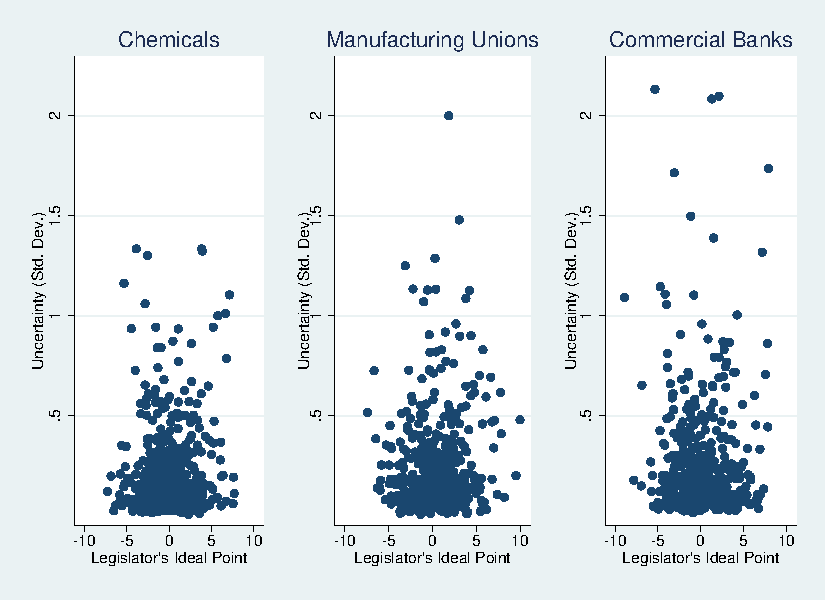
\includegraphics[height=3in, width=6.5in]{NSF_combined_graph.pdf}
\end{center}
\caption{Uncertainty by Industry\label{fig:combined}}
\end{figure}

Finally, we `turn on' the parameters for interest groups for each vote according to the data from Maplight, which includes a listing of the votes for which each interest group took a position. This produces estimates for how ``friendly'' or ``unfriendly'' each legislator is with respect to each interest group, as well as the unpredictability of his/her voting behavior when matters affecting that group are considered. In a preliminary run of this model with just ten interest groups (out of over 450) in the 112th Congress displayed in Figure~\ref{fig:combined}, we find that the chemical industry has the lowest average uncertainty (sd = 0.229); this is lower than the total uncertainty measure that can be interpreted as the standard left-right measure in ideal point models (sd = 0.233). The median group in terms of uncertainty is manufacturing unions (sd = 0.253), while construction equipment faced the highest uncertainty (sd = 0.285). This gives us a rich testing grounds for the model that is yet to be exploited.





%\subsection{Break Decision}

%\subsection{Uncertainty for Select Interest Groups}
%\label{sec:select}


\section{Conclusion}
\label{sec:concl}

We have characterized a model of vote buying in which there is uncertainty about the ideological positions of those whose votes are being bought, with information about this uncertainty symmetric among all players. This model describes some realistic aspects of lobbying and voting behavior: for instance, that lobbyists on both sides of an issue may be active at the same time, that moderate legislators and those about which there is average uncertainty receive more bribes than those that are ideologically extreme, and that ideal points gross of bribes need not be equalized.

An alternative characterization of the legislative process would be one in which (i) bills have a quality dimension (such as their technical merit, or their appropriateness for a given situation); and (ii) legislators have access to different pieces of information about the quality of these proposals. Adding common values and decentralized information to the analysis of the ratification of trade agreements will be one of the next steps in this project. Given the important set of governance characteristics identified in Mansfield and Milner (2012), we also look forward to taking advantage of what seems a rich opportunity to integrate important institutional variations into this modeling framework of endogenous lobbying with uncertainty.

We are also in the process of using this model to develop well-identified measures of legislative uncertainty. We expect this data will have a wide array of applications, such as exploring the links between policy uncertainty, the business cycle, and stock market volatility.

Having created these measures of political uncertainty---which are entirely new to the best of our knowledge---we will proceed to characterize this uncertainty across industries, as well as how it is related to lobbying, political contributions and voting behavior of legislators. First, we want to understand the patterns in these data in the context of the industry-relevant bills identified by Maplight as explained above.

We will use descriptive analysis as well as both standard parametric and non-parametric techniques such as density estimation to explore the relationships between the above variables of interest. We will begin with very basic questions such as whether distinct industries face varying levels of political uncertainty (see preliminary evidence in Figure~\ref{fig:combined}) and how those patterns may relate to the lobbying strategies they employ. The research agenda that is opened up by this modeling framework and the data to which it leads is extensive and provides for many exciting opportunities to better understand political and policy-making processes.

\section*{Appendix}
\label{sec:app}
\pdfbookmark{Appendix}{sec:appendix}
\noindent \textbf{\hypertarget{Pr_2NNB}{Proof of Proposition~\ref{prop:2NNB}}}: \\
Without loss of generality, assume that it is the legislators at $-\frac{1}{2}$ and $0$ that are bribed. The first order conditions with respect to the bribes for these two legislators are
	\begin{equation}
		\frac{e^{-X} + e^{-Z}}{\left(1+e^{-X}\right)\left(1+e^{-Z}\right)} \frac{e^{-Y}}{\left(1+e^{-Y}\right)^2}= \frac{1}{W_B}
	\end{equation}
	and
	\begin{equation}
		\frac{e^{-Y} + e^{-Z}}{\left(1+e^{-Y}\right)\left(1+e^{-Z}\right)} \frac{e^{-X}}{\left(1+e^{-X}\right)^2}= \frac{1}{W_B}
		\label{eq:base}
	\end{equation}
		
		Setting the left-hand size of these two equations equal to each other and simplifying,
		\[
		  \frac{e^{-Y} + e^{-Z}}{\left(1+e^{-Y}\right)\left(1+e^{-Z}\right)} \frac{e^{-X}}{\left(1+e^{-X}\right)^2}= \frac{e^{-X} + e^{-Z}}{\left(1+e^{-X}\right)\left(1+e^{-Z}\right)} \frac{e^{-Y}}{\left(1+e^{-Y}\right)^2}
		\]
		\[
		  \frac{e^{-X-Y} + e^{-X-Z}}{1+e^{-X}}= \frac{e^{-X-Y} + e^{-Y-Z}}{1+e^{-Y}}
		\]
		\[
		  e^{-X-Y} + e^{-X-Z} + e^{-X-2Y} +e^{-X-Y-Z}= e^{-X-Y} + e^{-Y-Z} + e^{-2X-Y} +e^{-X-Y-Z}
		\]
		\[
		  e^{-X-Z} +e^{-X-2Y}= e^{-Y-Z} +e^{-2X-Y}
		\]
		\[
		  e^{-Z} +e^{-2Y}= e^{X-Y-Z} +e^{-X-Y}
		\]
		\begin{equation}
		  e^{Y-Z} +e^{-Y}= e^{X-Z} +e^{-X}
			\label{eq:twoways}
		\end{equation}
   Equation~\ref{eq:twoways} can be rearranged into two similar forms. First:
		\[
		  e^{Y-Z} - e^{X-Z}= e^{-X} - e^{-Y}
		\]
		\begin{equation}
		  e^{Y} - e^{X}= e^Z\left(e^{-X} - e^{-Y}\right)
			\label{eq:1}
		\end{equation}
  	Second, multiplying through by zero:
	  \begin{equation}
		  e^{X} - e^{Y}= e^Z\left(e^{-Y} - e^{-X}\right)
			\label{eq:2}
		\end{equation}
		
In this case where the non-negativity constraint binds for the variable associated with $Z$, that is $b\left(-\frac{1}{2}\right)$, we know that $Z < 0$. Note that this is due to the construction of the problem. This means $e^Z < 1$. In this case,
	\begin{itemize}
		\item Equation~\ref{eq:1} is consistent with $X>Y>0$, $X>0>Y$, or $0>X>Y$.
		\item Equation~\ref{eq:2} is consistent with $Y>X>0$, $Y>0>X$, or $0>Y>X$.
	\end{itemize}
The second order conditions imply that both $X$ and $Y$ are positive, thus it must be that $X = Y > 0$ (see below). Note that once this is known, one can go back to, for instance, Equations~\ref{eq:base} and substitute for one of the variables. Given that $Z=0$, with a particular value of $\left(\alpha,W_B\right)$, the solution gives the values of the two relevant bribes.

\begin{comment}
\vskip.2in
\noindent \un{Second Order Conditions} \\
When one non-negativity constraint binds, the bordered Hessian is 4x4.\\
		$\left|\begin{tabular}{cccc}
			0 & $\frac{\partial g_1}{\partial b_{-\frac{1}{2}}}$ & $\frac{\partial g_1}{\partial b_0}$ & $\frac{\partial g_1}{\partial b_{\frac{1}{2}}}$ \\
			$\frac{\partial g_1}{\partial b_{-\frac{1}{2}}}$ & $\frac{\partial^2 L}{\partial b_{-\frac{1}{2}}^2}$ & $\frac{\partial^2 L}{\partial b_0\partial b_{-\frac{1}{2}}}$ & $\frac{\partial^2 L}{\partial b_{\frac{1}{2}} \partial b_{-\frac{1}{2}}}$  \\
			$\frac{\partial g_1}{\partial b_0}$ & $\frac{\partial^2 L}{\partial b_{-\frac{1}{2}} \partial b_0}$ & $\frac{\partial^2 L}{\partial b_0^2}$ & $\frac{\partial^2 L}{\partial b_{\frac{1}{2}}\partial b_0}$ \\
			$\frac{\partial g_1}{\partial b_{\frac{1}{2}}}$ & $\frac{\partial^2 L}{\partial b_{-\frac{1}{2}}\partial b_{\frac{1}{2}}}$ & $\frac{\partial^2 L}{\partial b_0 \partial b_{\frac{1}{2}}}$ & $\frac{\partial^2 L}{\partial b_{\frac{1}{2}}^2}$
		\end{tabular} \right|\\$
		
		\vskip.2in		
\noindent Evaluating the constraint terms, we have:\\
\begin{tabular}{cccc}
			0 & 0 & 0 & -1 \\
			0 & $\frac{\partial^2 L}{\partial b\left(-\frac{1}{2}\right)^2}$ & $\frac{\partial^2 L}{\partial b(0)\partial b\left(-\frac{1}{2}\right)}$ & $\frac{\partial^2 L}{\partial b\left(\frac{1}{2}\right)\partial b\left(-\frac{1}{2}\right)}$  \\
			0 & $\frac{\partial^2 L}{\partial b\left(-\frac{1}{2}\right)\partial b\left(0\right)}$ & $\frac{\partial^2 L}{\partial b(0)^2}$ & $\frac{\partial^2 L}{\partial b\left(\frac{1}{2}\right)\partial b\left(0\right)}$ \\
			-1 & $\frac{\partial^2 L}{\partial b\left(-\frac{1}{2}\right)\partial b\left(\frac{1}{2}\right)}$ & $\frac{\partial^2 L}{\partial b(0) \partial b\left(\frac{1}{2}\right)}$ & $\frac{\partial^2 L}{\partial b\left(\frac{1}{2}\right)^2}$
		\end{tabular}

\vskip.2in
The second order condition is on the last two principal minors. The last must be negative. The next to last should then be positive.

Let's begin with the next-to-last principle minor, which is the determinant of the 3x3 matrix that is the upper-lefthand corner of this matrix. This is
	\[
	  0 + 0 + 0 - \left[0 + 0 + (-1)(-1)\frac{\partial^2 L}{\partial b(0)^2} \right] = - \frac{\partial^2 L}{\partial b(0)^2}
	\]
\begin{itemize}
	\item First we need the determinant of the next-to-last principal minor, the . This determinant should be positive. We can use the trick by which one copies the first two rows to the right of the matrix and then multiplies down the columns to the right and up the columns to the right (these terms get a negative sign). Then the determinant is
	  \[
		  0 + 0 + 0 - \left[0 + 0 + (-1)(-1)\frac{\partial^2 L}{\partial b(0)^2} \right] = - \frac{\partial^2 L}{\partial b(0)^2}
		\]
		Because we need this to be positive, we need $\frac{\partial^2 L}{\partial b(0)^2} < 0$. This corresponds to the $X$ compositive variable, and happens only when $X$ is non-negative
	\item Second, we need the determinant of the last principal minor, which is the whole 4x4 matrix. This determinant can be simplified as follows:
		\[
		  0 \cdot \left|\text{something} \right| - (-1)\cdot 
			\left|\begin{array}{ccc}
				- 1 & \frac{\partial^2 L}{\partial b(0)\partial b\left(-\frac{1}{2}\right)} & \frac{\partial^2 L}{\partial b\left(\frac{1}{2}\right)\partial b\left(-\frac{1}{2}\right)}  \\
			0 & \frac{\partial^2 L}{\partial b(0)^2} & \frac{\partial^2 L}{\partial b\left(\frac{1}{2}\right)\partial b\left(0\right)} \\
			0 & \frac{\partial^2 L}{\partial b(0) \partial b\left(\frac{1}{2}\right)} & \frac{\partial^2 L}{\partial b\left(\frac{1}{2}\right)^2}
			\end{array} \right| + 0 \cdot \left|\text{something} \right| - 0 \cdot \left|\text{something} \right|
		\]
		\[ 
			=
			\left|\begin{array}{ccc}
				- 1 & \frac{\partial^2 L}{\partial b(0)\partial b\left(-\frac{1}{2}\right)} & \frac{\partial^2 L}{\partial b\left(\frac{1}{2}\right)\partial b\left(-\frac{1}{2}\right)}  \\
			0 & \frac{\partial^2 L}{\partial b(0)^2} & \frac{\partial^2 L}{\partial b\left(\frac{1}{2}\right)\partial b\left(0\right)} \\
			0 & \frac{\partial^2 L}{\partial b(0) \partial b\left(\frac{1}{2}\right)} & \frac{\partial^2 L}{\partial b\left(\frac{1}{2}\right)^2}
			\end{array} \right|
		\]
		\[
		  = - 1 \cdot \left|\begin{array}{cc}
			\frac{\partial^2 L}{\partial b(0)^2} & \frac{\partial^2 L}{\partial b\left(\frac{1}{2}\right)\partial b\left(0\right)} \\
			\frac{\partial^2 L}{\partial b(0) \partial b\left(\frac{1}{2}\right)} & \frac{\partial^2 L}{\partial b\left(\frac{1}{2}\right)^2}
			\end{array} \right|
		\]
		\[
		  = - 1 \cdot \left(
			\frac{\partial^2 L}{\partial b(0)^2} \frac{\partial^2 L}{\partial b\left(\frac{1}{2}\right)^2} - \left[\frac{\partial^2 L}{\partial b\left(\frac{1}{2}\right)\partial b\left(0\right)}\right]^2 \right)
		\]
		\[
		  = \left[\frac{\partial^2 L}{\partial b\left(\frac{1}{2}\right)\partial b\left(0\right)}\right]^2 - \frac{\partial^2 L}{\partial b(0)^2} \frac{\partial^2 L}{\partial b\left(\frac{1}{2}\right)^2}
		\]

  We need this determinant to be non-positive, that is
		\[
		  \frac{\partial^2 L}{\partial b(0)^2} \frac{\partial^2 L}{\partial b\left(\frac{1}{2}\right)^2} \geq \left[\frac{\partial^2 L}{\partial b\left(\frac{1}{2}\right)\partial b\left(0\right)}\right]^2 
		\]
	  The right hand side is positive because it's a square. Moreover, it is strictly positive because $\frac{\partial^2 L}{\partial b\left(\frac{1}{2}\right)\partial b\left(0\right)}$ is strictly positive: examine Equation~\ref{eq:xpartial}. Since $Z < 0$ in the case under examination, Equation~\ref{eq:xpartial} must be strictly positive. (This strengthens us from the negative semi-definite condition condition that supplies only a weak inequality).
		
		The left hand side must then be positive, and since we know that one term is positive from the previous principal minor result, the other must be positive as well. Thus both $X$ and $Y$ must be positive.
\end{itemize}
\end{comment}		
		
		
$\hfill\blacksquare$

\vskip.3in
\noindent \textbf{\hypertarget{Pr_3NNB}{Proof of Proposition~\ref{prop:3NNB}}}:
	
From the first order conditions, when $X$ and $Y$ are non-negative, it can be shown that the same set of inequalities as in the proof of Proposition~\ref{prop:2NNB} hold.

The second order conditions when there are no non-negativity constraints binding is simply that the 3x3 matrix of second derivatives be negative semi-definite. There are three conditions:
		\[
		  \frac{\partial^2 L}{\partial b\left(-\frac{1}{2}\right)^2} \left\{\frac{\partial^2 L}{\partial b(0)^2} \frac{\partial^2 L}{\partial b\left(\frac{1}{2}\right)^2} - \left[\frac{\partial^2 L}{\partial b\left(\frac{1}{2}\right)\partial b\left(0\right)}\right]^2 \right\} \leq 0
		\]
		\[
		  \frac{\partial^2 L}{\partial b(0)^2} \frac{\partial^2 L}{\partial b\left(\frac{1}{2}\right)^2} - \left[\frac{\partial^2 L}{\partial b\left(\frac{1}{2}\right)\partial b\left(0\right)}\right]^2 \geq 0
		\]
		\[
		  \frac{\partial^2 L}{\partial b\left(\frac{1}{2}\right)^2} \leq 0
		\]
		The last one says that $Y$ must be non-negative. The first and second together say that $Z$ must be non-negative.
	
	If we combine the requirement that $Y$ must be non-negative combined with the inequalities cited above, then we must have $X=Y > 0$. A similar logic can be used to show that we must have $X=Z > 0$. Combining these two expressions leads to the desired result: $X=Y=Z >0$. $\hfill\blacksquare$

\vskip.3in
\noindent \textbf{\hypertarget{Pr_1NNB}{Proof of Proposition~\ref{prop:1NNB}}}: \\
When Vote Buyer B bribes just one legislator, two non-negativity constraints are binding and only one first order conditions holds with equality with the Lagrange multiplier equaling zero. We can easily solve this first order condition to find the value of the bribe. What determines which legislator is bribed is which legislator's ideal point distribution has the most mass near zero, as moving this individual has the greatest impact on total probability of winning the issue. $\hfill\blacksquare$


\vskip.3in
\noindent \textbf{\hypertarget{Pr_bothbribe}{Proof of Proposition~\ref{prop:bothbribe}}}: \\
Take the following example. Let $\al=0$ so that the means of the ideal point distribution for the three legislators are $-\frac{1}{2}$, $0$ and $\frac{1}{2}$. Let the willingness-to-pay parameters be $W_A = 6$ and $W_B = 8$. And let the scale parameters for the legislators at $0$ and $\frac{1}{2}$ be 1 and $s_{-\frac{1}{2}} = 1.1$.

In this example, the optimal bribe offer function for Vote Buyer $A$ is to offer nothing to the legislators at $0$ and $\frac{1}{2}$ and $a_{-\frac{1}{2}}=0.4$. Vote Buyer $B$ responds by offering nothing to the legislators at $-\frac{1}{2}$ and $\frac{1}{2}$ and $b_0 = 0.21$ to the legislator at zero. The final gross positions of the mean parameters for the three legislators are, from left to right, $\left\{ -0.1, -0.21, 0.5 \right\}$, with one legislator each being lobbied in each direction.


\newpage
\section*{References}
\pdfbookmark{References}{sec:refs}

\begin{list}{}{\setlength{\leftmargin}{0.3in}\setlength{\rightmargin}{0.0in}\setlength{\itemindent}{-0.3in}\setlength{\itemsep}{0.0in}}


\item Ansolabehere, S., J. de Figueiredo, and J. Snyder Jr. (2003), ``Why Is There so Little Money in U.S. Politics?,'' {\em Journal of Economic Perspectives}, 17, 105-130.

\item Bafumi, J., Gelman, A., Park., D, Kaplan, N., 2005. Practical Issues in Implementing and Understanding Bayesian Ideal Point Estimation. Political Analysis 13, 171-187.
	
\item Banks, J. S., (2000), ``Buying Supermajorities in Finite Legislatures.'' {\em The American Political Science Review} 94, 677-681.

\item Becker, G., (1983), ``A Theory of Competition among Interest Groups for Political Influence.'' {\em Quarterly Journal of Economics} 98, 371-400.

\item Bombardini, M. (2008), ``Firm Heterogeneity and Lobby Participation,'' {\em Journal of International Economics}, 75, 329-348.

\item Bombardini, M., and F. Trebbi (2012): ``Competition and Political Organization: Together or Alone in Lobbying for Trade Policy?'' {\em Journal of International Economics}, 87, 18-26.

\begin{sloppypar}	
	\item Buzard, K., 2016. Trade Agreements in the Shadow of Lobbying. Available at: \url{http://papers.ssrn.com/sol3/papers.cfm?abstract_id=2168522}.
\end{sloppypar}

\item Clinton, J., Jackman, S., and D. Rivers, (2004): ``The Statistical Analysis of Roll Call Data.'' {\em American Political Science Review}, 98, 355-370.

\item Coates, D., Ludema, R., 2001. A Theory of Trade Policy Leadership. Journal of Development Economics 65, 1-29.
	
\item Dal Bo, E. (2007): ``Bribing Voters.'' {\em American Journal of Political Science} 51, 789-803.

\item Dekel, E., Jackson, M., Wolinsky, A. (2005): {\em Vote Buying.} Unpublished manuscript, Caltech.

\item Gawande, K., Krishna, P., Olarreaga, M., 2009. What Governments Maximize and Why: The View from Trade. International Organization 63, 491-532.

\item Goldberg, P. and G. Maggi (1999): ``Protection for Sale: An Empirical Investigation,'' {\em American Economic Review}, 89, 1135-1155.

\item Groseclose, T., Snyder, J. M. (1996): ``Buying Supermajorities.'' {\em American Political Science Review} 90, 303-315.

\item Grossman, G. and E. Helpman (1994): ``Protection for Sale,'' {\em The American Economic Review}, 84, 833-850.

\item Grossman, G., Helpman, E., 1995a. The Politics of Free-Trade Agreements. The American Economic Review 85, 667-690.

\item Grossman, G., Helpman, E., 1995b. Trade Wars and Trade Talks. The Journal of Political Economy 103, 675-708.

\item Grossman, G. and E. Helpman (2005): ``A Protectionist Bias in Majoritarian Politics,'' {\em The Quarterly Journal of Economics}, 120, 1239-1282.

\item Henisz, W. and E. Mansfield (2006), ``Votes and Vetoes: The Political Determinants of Commercial Openness,'' {\em International Studies Quarterly}, 50, 189-211.

\item Kibris, A. (2012), ``Uncertainty and Ratification Failure,'' {\em Public Choice}, 150, 439-467.

\item Laffont, J., Tirole, J. (1994): ``A Theory of Incentives in Procurement and Regulation.'' Cambridge: MIT Press.

\item Lake, J., 2015. Revisiting the link between PAC Contributions and Lobbying Expenditures. European Journal of Political Economy 37, 86-101.

\item Laver, M. and K. Shepsle (1991), ``Divided Government: America is Not `Exceptional','' {\em Governance: An International Journal of Policy and Administration}, 4, 250-269.

\item Le Breton, M. and F. Salanie (2003), ``Lobbying under political uncertainty,'' {\em Journal of Public Economics}, 87, 2589-2610.

\item Le Breton, M. and V. Zaporozhets (2007), ``Legislative Lobbying under Political Uncertainty,'' Available at SSRN: \url{http://ssrn.com/abstract=1024686}.

\item Mansfield, E., Milner, H., 2012. Votes, Vetoes, and the Political Economy of International Trade Agreements. Princeton and Oxford: Princeton  University Press.

\item Peltzman, S. (1976), ``Toward a More General Theory of Regulation.'' {\em Journal of Law and Economics} 19, 211-248.

\item Poole, K. T. (2005), ``Spatial Models of Parliamentary Voting.'' New York: Cambridge University Press.

\item Saiegh, S. (2009), ``Political  Prowess or Lady Luck? Evaluating Chief Executives' Legislative Success Rates,'' {\em The Journal of Politics}, 71, 1342-1356.

\item Saiegh, S. (2011) ``Ruling by Statute: How Uncertainty and Vote-Buying Shape Lawmaking.'' New York: Cambridge University Press.

\item Stigler, G. (1975) ``The Citizen and the State: Essays on Regulation.'' Chicago: Chicago University Press.

\end{list}

\end{document}